\documentclass[10pt,letter]{article}
\usepackage{graphicx}

\author{Dustin Lang}
\title{Design of a Deblender}

\begin{document}
\maketitle

\section{Introduction}

This document describes the iterative design of a deblender through
experiments.  It is presented as a sequence of refinements guided by
looking at the results on real data.


%  hg clone hsc-gw2.mtk.nao.ac.jp://ana/hgrepo/supaDb
%  python bin/supa_ingest.py ham.sql3 data/SUP_20{09,10}.txt
%  (echo "# id filter ra decl expTime type mode object"; sqlite3 ../supaDb/ham.sql3 "select id,filter,ra,decl,expTime,type,mode,object from suprimecam where type='OBJECT' and exptime>119 and filter like 'W%' and mode like 'IMAG%';") > ham.txt
%  python select.py
%
% obj SDSS1115 : 79 exposures
% Filter W-S-G+ with 4 exposures, total exptime 1200.0 ( [ 300.] )
% Filter W-S-I+ with 8 exposures, total exptime 1920.0 ( [ 240.] )
% Filter W-S-R+ with 7 exposures, total exptime 2100.0 ( [ 300.] )
% Filter W-S-Z+ with 60 exposures, total exptime 7200.0 ( [ 120.] )
% 
% Arbitrarily choose visit 108792 -- G-band


\section{Starting ansatz}

The initial ansatz, due to Robert Lupton \cite{rhldeblend} and
implemented in the SDSS \emph{Photo} software, is that astronomical
sources have two-fold rotational symmetry and a peak in the center.
This is a fiendishly clever observation that will take us a long way.
We will begin by describing the SDSS deblending algorithm built around
this ansatz, sweeping several details under the rug until later.

The SDSS deblender takes as input a ``footprint'' and a set of
``peaks''.  A footprint is a connected set of pixels that are
significantly above a detection threshold, grown by a margin of about
the size of the PSF.  ``Peaks'' are just what you expect:
(PSF-convolved) pixels significantly higher than their neighbors.

For each peak, the SDSS deblender builds a ``template'' image by
applying the symmetry ansatz.  Starting from the peak pixel, at
position $(p_x,p_y)$, the template at positions $(p_x + dx, p_y +
dy)$, $(p_x - dx, p_y - dy)$ contains the \emph{minimum} of those two
pixel values.  The difference between the minimum and the value at the
higher pixel is presumed to be due to other blended sources.

Having built a template for each peak, the SDSS deblender computes the
least-squares \emph{weight} for each template to best reproduce the
observed image.

Finally, the counts in each image pixel are split between the
templates covering that pixel in proportion to the values of the
templates.

\begin{figure}
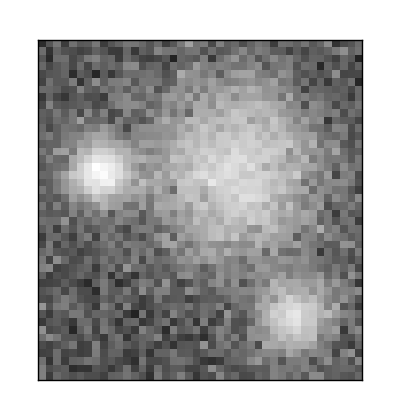
\includegraphics[width=0.1\textwidth]{design-image-0828} \\
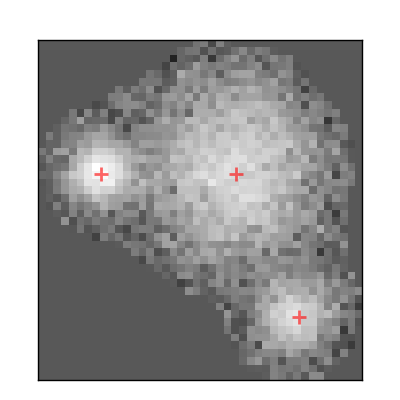
\includegraphics[width=0.1\textwidth]{design-parent-0828} \\
%
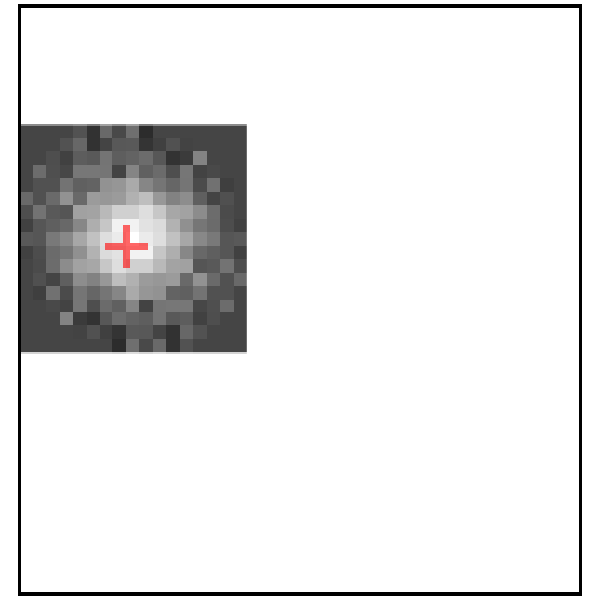
\includegraphics[width=0.1\textwidth]{design-0828-t0}%
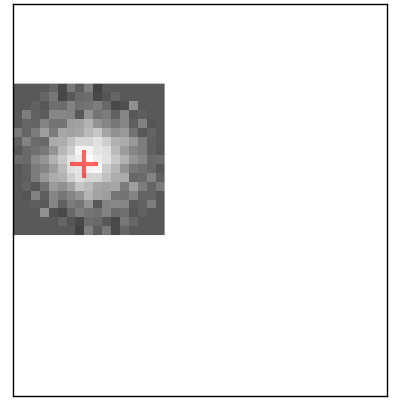
\includegraphics[width=0.1\textwidth]{design-0828-t1}%
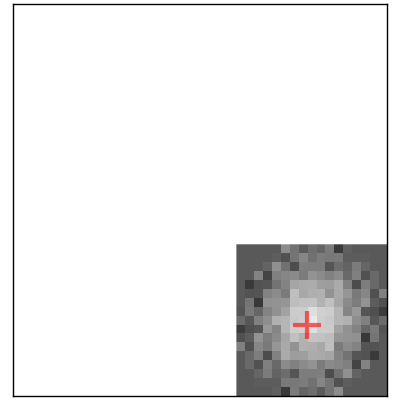
\includegraphics[width=0.1\textwidth]{design-0828-t2} \\
%
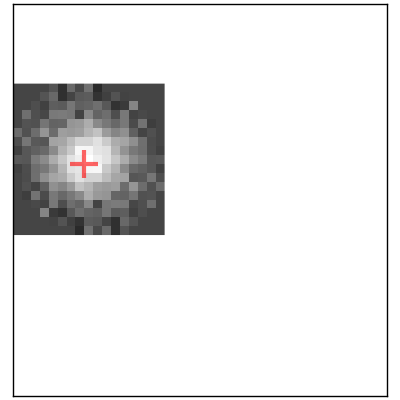
\includegraphics[width=0.1\textwidth]{design-0828-tw0}%
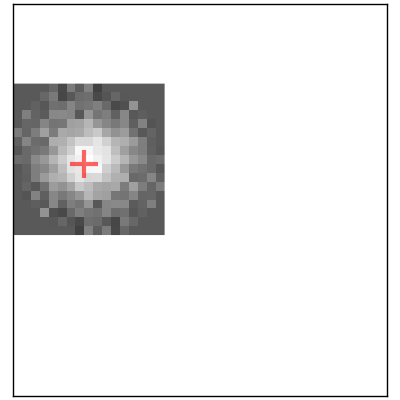
\includegraphics[width=0.1\textwidth]{design-0828-tw1}%
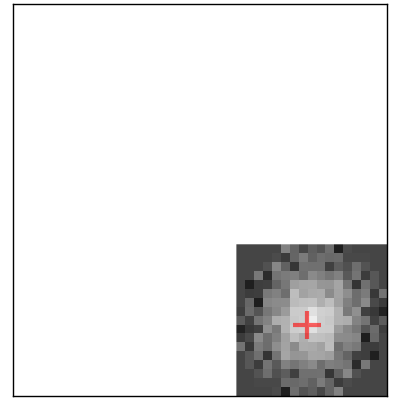
\includegraphics[width=0.1\textwidth]{design-0828-tw2} \\
%
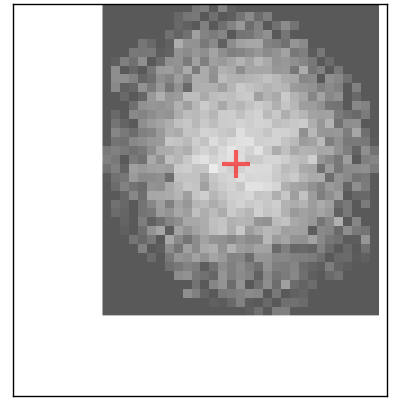
\includegraphics[width=0.1\textwidth]{design-0828-h0}%
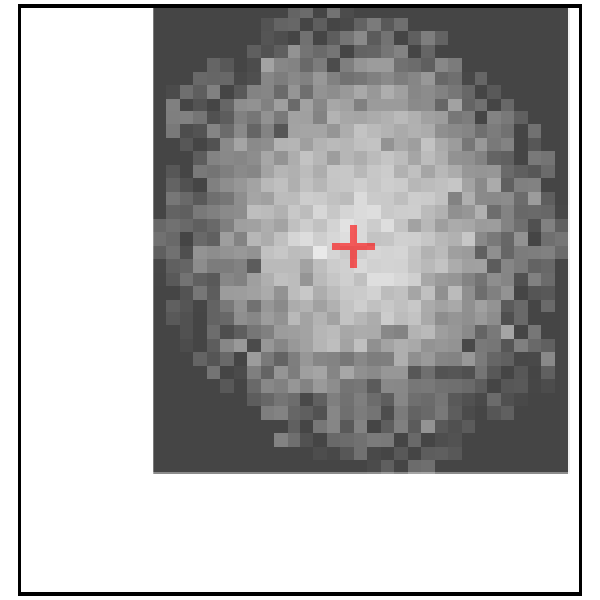
\includegraphics[width=0.1\textwidth]{design-0828-h1}%
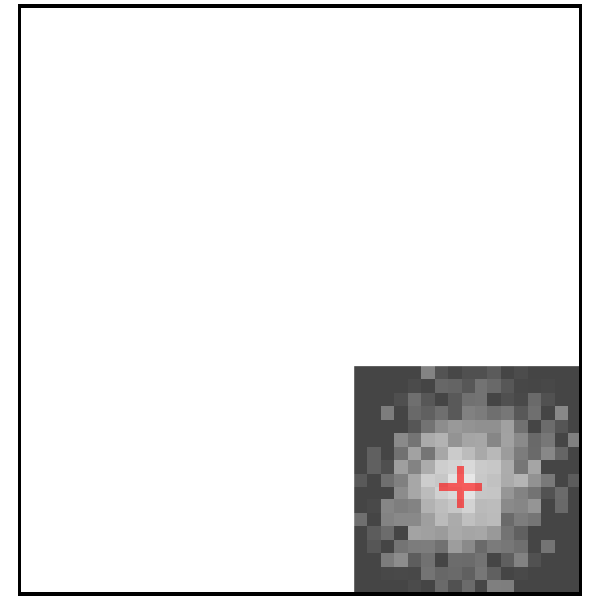
\includegraphics[width=0.1\textwidth]{design-0828-h2} \\
\end{figure}


\end{document}

